\chapter{Design and Implementation of \RS{} System }
\label{c:OverviewRS}
Three major components in \RS{}: 
\begin{itemize}
    \item \textbf{Offline} Compiler: \textit{llvm-rs-cc} (stands for \textbf{LLVM} \textbf{RS} \textbf{C} \textbf{C}ompiler)
    \item \textbf{Online} JIT Compiler: \textit{libbcc.so} (stands for \textbf{B}i\textbf{C}ode \textbf{C}ompiler)
    \item \RS{} \textbf{Runtime}: \textit{libRS.so}
\end{itemize}
When you build your RS project, Android SDK will use \slang{} to compile your .rs file to .bc file (LLVM bitcode), plus reflection. (We will discuss reflection later in section \ref{ss:Bridge}.) The .bc file will be packaged with Java files and other application resources into a APK file. Once you launch the RS applicaiotn after installation, \bcc{} would be invoked to just-in-time compile the bitcode. \RS{} runtime then supports the execution of \Core{}. 

\section{\RS{}~Directory \lmr{\textsc{Structure}}}
\label{s:RDS}

Let's take a overview on the directories coverd in this thesis.
\begin{itemize}
	\item \hyperref[ss:JavaClient]{\textbf{Java SDK}} (\Client{} side):\\
	        You can refer to the \href{http://developer.android.com/reference/android/renderscript/package-summary.html}{offical document} for API usage.\\
\verb|<FRAMEWORKS_BASE>/graphics/java/android/renderscript|\\
	\item \hyperref[ss:NativeEngine]{\textbf{Native Engine}} (\Core{} side):\\
\verb|<FRAMEWORKS\_BASE>/libs/rs|
	\item \hyperref[ss:Bridge]{\textbf{JNI Bridge}}:\\
\verb|<FRAMEWORKS_BASE>/graphics/jni|
	\item \textbf{RS Graphics Commands and API}:\\
\verb|out/target/product/<DEV>/obj/SHARED_LIBRARIES/libRS_intermediates/|
	\item \textbf{Reflected Java Code}:\\
\verb|<APP_intermediates>/src/renderscript/res/raw|\\
\verb|<APP_intermediates>/src/renderscript/src/com/android/fountain|\footnote{Path of <APP\_intermediates>: <ANDROID\_ROOT>/out/target/common/obj/APPS/APPNAME\_intermediates/}
	\item \textbf{Compiled bitcode}:\\
\verb|<APP_intermediates>/src/renderscript/res/raw|
\end{itemize} 

\subsection{Native Engine}
\label{ss:NativeEngine}

Native Engine means the \RS{} runtime, \textit{libRS.so}, and the source is located on \verb|frameworks/base/libs/rs|. All real \RS{} implementation is there, including RS graphics-specific header\footnote{in scriptc/}.

Some key features of the native \RS{} libraries include:
\begin{enumerate}
\item A large collection of math functions with both \textbf{scalar} and \textbf{vector} typed overloaded versions of many common routines. Operations such as adding, multiplying, dot product, and cross product are available.
\item Conversion routines for primitive data types and vectors, matrix routines, date and time routines, and graphics routines.
\item Logging functions
\item Graphics rendering functions
\item Memory allocation request features
\item Data types and structures to support the \RS{} system such as Vector types for defining two-, three-, or four-vectors.
\end{enumerate}

\subsection{Java Client}
\label{ss:JavaClient}
All application is wrapped in Java code, of course, RS application is not the exception. Java Client takes charge of UI handling, collaborates with other SDK code, and do partial initialization of RS application.
Android Developer will not be able to get accesses to \Core{}. Only Java SDK code is permitted to use, so even RS object(see sec \ref{s:RSObject}) should be allocated by invoking Java SDK.

Two major \RS{} context classes of Java Client: 
\begin{itemize}
\item \textbf{RenderScript} is for a compute RS script.
\item \textbf{RenderScriptGL} is for a graphics RS script.\\\RS{} provides a number of graphics APIs for hardware-accelerated 3D rendering. The \RS{} graphics APIs include a stateful context, RenderScriptGL that contains the current rendering state. The primary state consists of the objects that are attached to the rendering context, which are the graphics \RS{} and the four program types.\footnote{The four program types mirror a traditional graphical rendering pipeline and are: (1)Vertex; (2)Fragment; (3)Store; and (4)Raster.} Graphical scripts have more properties beyond a basic computational script, and they call the 'rsg'-prefixed functions defined in the rs\_graphics.rsh header file. 
\end{itemize}
With above two classes, you could bind to the reflected \RS{} class, so that the \RS{} context knows what its corresponding native \RS{} is. If you have a graphics \RS{} context, you can also specify a variety of Programs (stages in the graphics pipeline) to tweek how your graphics are rendered. A graphics \RS{} context also needs a surface to render on, \textit{RSSurfaceView}, which gets passed into RSSurfaceView's constructor. 

The Android system APIs are broken into a few main groups\cite{package-summary}:
\begin{itemize}
\item \textbf{Allocation APIs} are used internally by the system for memory allocation. They are used by the classes that are generated by the build tools:
\item \textbf{Data Types} are used by the classes that are generated by the build tools. They are the reflected counterparts of the native data types that are defined by the native RS APIs and used by your RS code. 
\item \textbf{Graphics APIs} are specific to graphics \RS{} and support a typical rendering pipeline.
\end{itemize}
\begin{center-table}
	\label{t:prefix-table}
	\caption{Major gourps of APIs}
	\renewcommand{\arraystretch}{1.0}
	%\newcolumntype{C}{>{\centering}X}
	\begin{tabularx}{300pt}{|c|X| }
		\hline
		\multirow{1}{*}{\textbf{Allocation}} &
		Allocation, Element, Type, Script 
		\\ \hline\hline
		%------------------------------
		\multirow{6}{*}{\textbf{Data Types}} &
        Byte2, Byte3, and Byte4\\ &
        Float2, Float3, Float4\\ &
        Int2, Int3, Int4\\ &
        Long2, Long3, Long4\\ &
        Matrix2f, Matrix3f, Matrix4f\\ &
        Short2, Short3, Short4
        \\ \hline\hline
		%------------------------------
		\multirow{4}{*}{\textbf{Graphics}} &
		Mesh\\&
		ProgramFragment, ProgramRaster\\&
		ProgramStore, ProgramVertex\\&
		RSSurfaceView
		\\ \hline
		%------------------------------
	\end{tabularx}
\end{center-table}

\subsection{Bridge in between}
\label{ss:Bridge}
\textit{Bridge} provides the entry points into the native code, enabling the Android system to give high level commands like, "rotate the view" or "filter the bitmap" to \textit{Client}, which does the heavy lifting. To accomplish this, you need to create logic to hook together all of these ones so that they can correctly communicate.

\textit{libRS.so} is written in C++, so the way to communicate beteen \textbf{Core} and \textbf{Client} is using \textit{JNI}. This mapping is done in libjni.so. The mapping function table is as below:
\begin{lstlisting}[style=nonumbers] 
static JNINativeMethod methods[] = {   
    ...
{"rsnContextBindRootScript",      "(II)V", (void*)nContextBindRootScript },
{"rsnContextBindProgramStore",    "(II)V", (void*)nContextBindProgramStore },
{"rsnContextBindProgramFragment", "(II)V", (void*)nContextBindProgramFragment },
{"rsnContextBindProgramVertex",   "(II)V", (void*)nContextBindProgramVertex },
{"rsnContextBindProgramRaster",   "(II)V", (void*)nContextBindProgramRaster },
    ...
}
\end{lstlisting}

Besides JNI, reflected Java classes work as \Bridge{}.

\paragraph{Reflection} generates the class named \textit{ScriptC\_FILENAME.java} from a \RS{} file that has the .rs file extension. 
\textit{ScriptC\_fountain.java} which is the reflective version of the \RS{} and contains the entry points into the fountain.rs native code. This class does not appear until you run a build.

Any non-static, global \RS{} variables are reflected into \textit{ScriptC\_FILENAME.java}. Accessor methods are generated, so \textit{Client} can access the values. The get method comes with a one-way communication restriction. \textit{Client} always caches the last value that is set and returns that during a call to a get method. If the native \RS{} code changes the value, the change does \textbf{not} propagate back to \textit{Client}. If the global variables are initialized in the native \RS{} code, those values are used to initialize the corresponding values in \textit{Client}. If global variables are marked as \verb|const|, then a set method is not generated.

Structs are reflected into their own classes, one for each struct, into a class named \textit{ScriptField\_STRUCT.java} of type \verb|Script.FieldBase|.

Global pointers have a special property. They provide attachment points where \textit{Client} can attach allocations. If the global pointer is a user defined structure type, it must be a type that is legal for reflection (primitives or \RS{} data types). \textit{Client} can call the reflected class to allocate memory and optionally populate data, then attach it to the \RS{}. For arrays of basic types, the procedure is similar, except a reflected class is not needed. \RS{} should not directly set the exported global pointers.


\subsection{Subtle Function Name}
\label{ss:Stupid}

\begin{itemize}
	\item \textbf{android\_renderscript\_RenderScript.cpp}(It's auto-generated):
		\begin{lstlisting}[style=nonumbers]
{"rsnScriptCCreate", "(ILjava/lang/String;)I", (void*)nScriptCCreate }
Java’s native method				           Native method but has JNI
		\end{lstlisting} 
	\item BTW, in the same file we have:
		\begin{lstlisting}[style=nonumbers]
static jint nScriptCCreate(JNIEnv *_env, jobject _this,
{
	RsContext con, jstring resName)
	LOG_API("nScriptCCreate, con(%p)", con); 
	const char* resNameUTF = _env->GetStringUTFChars(resName, NULL); 
	return (jint)rsScriptCCreate(con, resNameUTF); 
	// Note: rsScriptCCreate is created based on rs.spec.
	// It will just call rsi_ScriptCCreate
}
		\end{lstlisting}
	\item RenderScript.java:
			\begin{lstlisting}[style=nonumbers]
native int rsnScriptCCreate(int con, String val); 
synchronized int /*Better name: NScriptCCreate*/ nScriptCCreate(String { 			
	// Terrible naming. This "nScriptCCreate" is different from
	// the (void*)nScriptCCreate above. This "nScriptCCreate" is invoked // ScriptC.java
	return rsnScriptCCreate(mContext, val);
}				           
			\end{lstlisting} 
\end{itemize} 


\section{\RS{} Commands}
\label{s:RSCommands}
RS Commands to JNI: They are generated at Build Time. Figure \ref{fig:rsg_generator} shows how it works.

\textit{spec.l} and \textit{spec.h} are files for \textbf{rsg\_generator}\footnote{g stands for "g"raphics.} to scan \textit{rs.spec} so that it could generate RS Commands related implementation, header files, etc. (Output path see sec.\ref{s:RDS})
\begin{center-figure}
	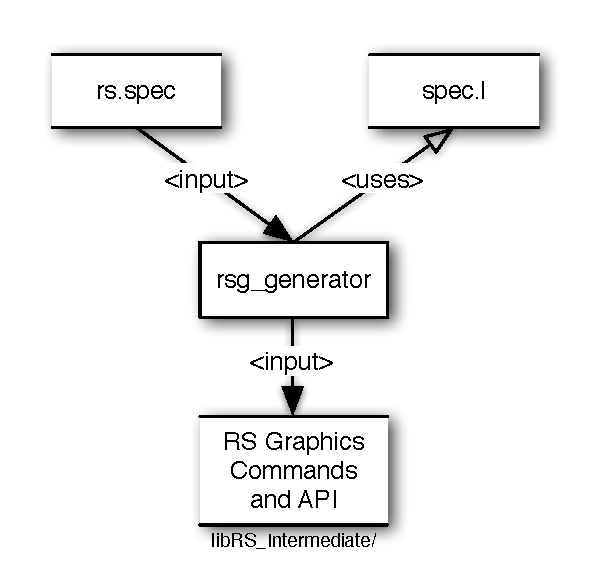
\includegraphics[scale=0.8]{fig/rsg_generator.eps}
	\caption{RS graphics API generator}
	\label{fig:rsg_generator}
\end{center-figure}

\subsection{API Prefix}
\label{ss:Prefix}
The star marks in the following table usually follow the rules [Class name][Action]. Take "rsi\_ScriptSetClearDepth()" as example, [Class name] is "Script" and [Action] is "SetClearDepth". Thus, its implementation would be found under frameworks/base/libs/rs (libRS.so, since its prefix is rsi\_) in rsScript.cpp (by [Class name].)

% Footnote in table:
% manually add a footnote which exists inside the table
\addtocounter{footnote}{1}
\footnotetext[\value{footnote}]{For example, rsi\_ScriptCreate(), which will call \textit{ScriptCState::runCompiler()}}
\addtocounter{footnote}{1}
\footnotetext[\value{footnote}]{The rs*() finally routes here}
\addtocounter{footnote}{1}
\footnotetext[\value{footnote}]{an integer constant} 
\addtocounter{footnote}{1}
\footnotetext[\value{footnote}]{rs*()->...->rsp\_*()->rsi\_*(), \textit{rsgApiReplay.cpp}}
% reset the counter to the first footnote's value
\addtocounter{footnote}{-4}
 
\begin{center-table}
	\label{t:prefix-table}
	\caption{RS API Prefix Table}
	\renewcommand{\arraystretch}{1.0}
	\begin{tabularx}{\textwidth}{| c | X | X |}
		\hline
		\multicolumn{1}{|c|}{\textbf{Component}} &
		\multicolumn{1}{c|}{\textbf{Prefix}} &
		\multicolumn{1}{c|}{\textbf{Comment}} \\
		\hline\hline
		\multirow{3}{*}{libRS.so} & % Component
		 &% Prefix
		File names are prefixed with rs* \\ % Comment
		\cline{2-3}
		
		 &   % Component
		rsi\_*()\footnotemark  & % Prefix
		RS API real implementation \footnotemark 
		\\ % Comment

        & % Component
		rsa\_*() &% Prefix
		RS allocation API  \\ % Comment

		\hline\hline
% ---------------------------------------------------------------------
		\multirow{4}{*}{RS Command} & % Component
		rs*()\footnotemark & % Prefix
		the commands, \textit{rsgApi.cpp}  \\ % Comment
		\cline{2-3}
		& % Component
		RS\_CMD\_* & % Prefix
		parameter data structure for the command \\ % Comment
		\cline{2-3}
		& % Component
		RS\_CMD\_ID\_* & % Prefix
		command ID  \footnotemark 
		\\% Comment
		\cline{2-3}
		& % Component
		rsp\_*  & % Prefix
		playback function \footnotemark % Comment
		\\
		\hline\hline
% ---------------------------------------------------------------------
		JNI & % Component
		n*() & % Prefix
		\textbf{n} stands for native % Comment
		\\
		\hline
	\end{tabularx}
\end{center-table}

We illustrate the usage of each kind of prefix in Figure \ref{fig:CommandQueuePushPop}. Why not call rsi\_ScriptSetVarF(...)? It's because that only ID and a pointer could be pulled out of a command. To call rsi\_ScriptSetVarF(...), we need exact arguments. Hence we do a casting with known structure information in \textit{rsgApiStruct.h}.
\begin{center-figure}
	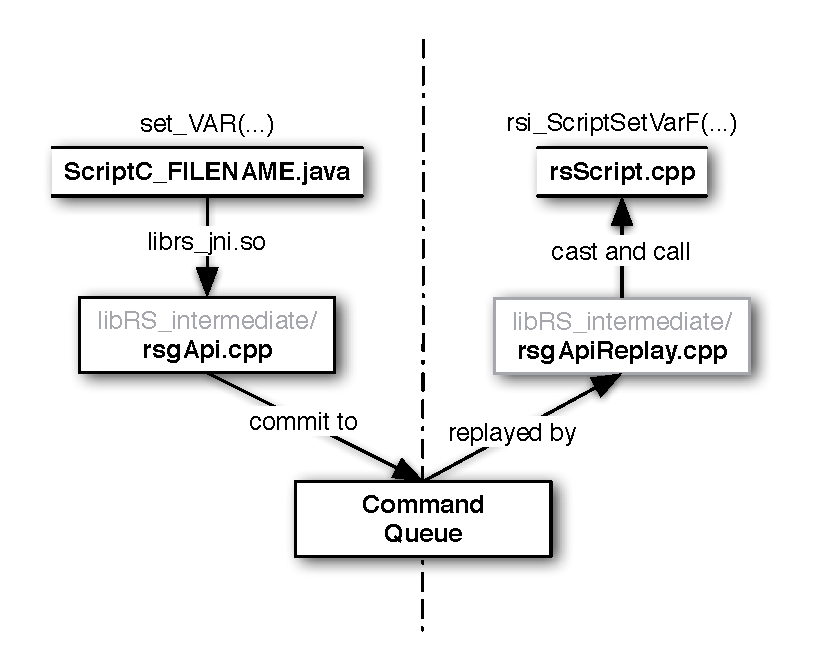
\includegraphics[scale=0.8]{fig/CommandQueuePushPop.eps}
	\caption{A command set\_VAR(value) called from \Client{} and executed in \Core{}.}
	\label{fig:CommandQueuePushPop}
\end{center-figure}

\section{The Fountain RS Application}
\label{s:FountainWorkflow}
For an example of \RS{} in action, see the 3D carousel view in the Android 3.0 versions of Google Books and YouTube or install the \RS{} sample applications that are shipped with the SDK.

In this thesis, we take \Fountain{} for instance. \Fountain{} acts just like its name. If any touches on screen, \Fountain{} spraies out points in direct proportion of the pressure.

In \Fountain{}, each file has its own distinct use. The following files comprise the main parts of the sample and demonstrate in detail how the sample works:
\begin{itemize}
\item \textbf{Fountain.java} ---  The main Activity for the application. This class is present to provide Activity lifecycle management. It mainly delegates work to FountainView, which is the \RS{} surface that the sample actually draws on.
\item \textbf{FountainView.java} --- The \RS{} surface that the graphics render on. If you are using \RS{} for graphics rendering, you must have a surface to render on. If you are using it for computatational operations only, then you do not need this.
\item \textbf{FountainRS} --- The class that calls the native \RS{} code through high level entry points that are generated by the Android build tools.
\item \textbf{fountain.rs} --- The \RS{} native code that draws the text on the screen.
\end{itemize}

The <project\_root>/gen directory contains the reflected layer classes that are generated by the Android build tools. You will notice a ScriptC\_fountain class, which is the reflective version of the \RS{} and contains the entry points into the fountain.rs native code. This file does not appear until you run a build.

\paragraph{ScriptC\_fountain}
This class is generated by the Android build tools and is the reflected version of the fountain.rs \RS{}. It provides a a high level entry point into the fountain.rs native code by defining the corresponding methods that you can call from the traditional framework APIs.

\paragraph{fountain.bc bitcode}
This file is the intermediate, platform-independent bitcode that gets compiled on the device when the \RS{} application runs. It is generated by the Android build tools and is packaged with the .apk file and subsequently compiled on the device at runtime. This file is located in the <project\_root>/res/raw/ directory and is named rs\_FILENAME.bc. You need to bind these files to your \RS{} context before call any \RS{} code from your Android application. You can reference them in your code with R.id.rs\_FILENAME.

\paragraph{FountainView class}
This class represents the Surface View that the \RS{} graphics are drawn on. It does some administrative tasks in the ensureRenderScript() method that sets up the \RS{} system. This method creates a RenderScriptGL object, which represents the context of the \RS{} and creates a default surface to draw on (you can set the surface properties such as alpha and bit depth in the RenderScriptGL.SurfaceConfig class ). When a RenderScriptGL is instantiated, this class calls the HelloRS class and creates the instance of the actual \RS{} graphics renderer.
This class also handles the important lifecycle events and relays touch events to the \RS{} renderer. When a user touches the screen, it calls the renderer, FountainRS and asks it to draw the text on the screen at the new location.

\paragraph{FountainRS class}
This class represents the \RS{} renderer for the FountainView Surface View. It interacts with the native \RS{} code that is defined in fountain.rs through the interfaces exposed by ScriptC\_fountain. To be able to call the native code, it creates an instance of the \RS{} reflected class, ScriptC\_fountain. The reflected \RS{} object binds the \RS{} bitcode (R.raw.fountain) and the \RS{} context, RenderScriptGL, so the context knows to use the right \RS{} to render its surface.


\subsection{Root Script}
\label{ss:RootScript}
Root Script means a script with root function:
The main working function of the graphics \RS{} is the code that is defined in the root() function. The root() function is called each time the surface goes through a frame refresh.

\paragraph{root()} This function is the default worker function for this \RS{} file. For graphics \RS{} applications, like this one, the \RS{} system expects this function to render the frame that is going to be displayed. It is called every time the frame refreshes. The root() function for the fountain.rs script moves all pixels down to simulate the dropping \textbf{every 1ms}.

\begin{lstlisting}
int root() {
    float dt = min(rsGetDt(), 0.1f);
    rsgClearColor(0.f, 0.f, 0.f, 1.f);
    const float height = rsgGetHeight();
    const int size = rsAllocationGetDimX(rsGetAllocation(point));
    float dy2 = dt * (10.f);
    Point_t * p = point;

    for (int ct=0; ct < size; ct++) {
        p->delta.y += dy2;
        p->position += p->delta;
        if ((p->position.y > height) && (p->delta.y > 0)) {
            p->delta.y *= -0.3f;
        }   
        p++;
    }   

    rsgDrawMesh(partMesh);
    return 1;
}
\end{lstlisting} 

\paragraph{init()} This function is called once for each instance of this \RS{} file that is loaded on the device, before the script is accessed in any other way by the \RS{} system. The init() is ideal for doing one time setup after the machine code is loaded such as initializing complex constant tables. The init() function for the fountain.rs script sets the initial location of the text that is rendered to the screen:

\subsection{old-version, libacc}
\label{ss:libacc}
As we mentioned in the begining of this chapter, there are three major components in \RS{} system. In the earlier version of Android (v2.0 - v2.3.3), only two component in \RS{} system: (1) online compiler libacc; and (2) \RS{} runtime.

libacc is a small C compiler, not like libbcc which compiles bitcode, it compiles normal native C code. Figure \ref{fig:workflow_libacc} shows the old workflow. We could found that the old workflow is difficult to use and debug. Not until running the application can we find the compile error.

\begin{center-figure}
	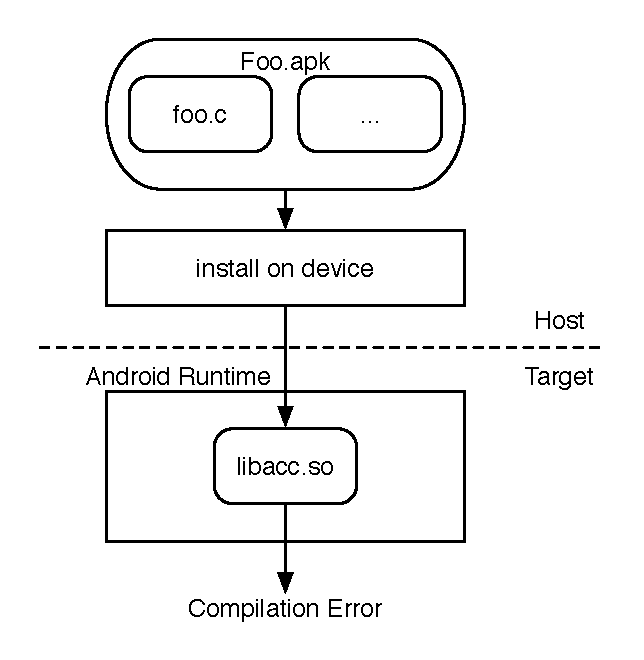
\includegraphics[scale=0.8]{fig/libacc_workflow.eps}
	\caption{workflow of libacc}
	\label{fig:workflow_libacc}
\end{center-figure}

\subsection{new-version, libbcc}
\label{ss:libbcc}
To overcome those shortages, Google replaces libacc with \textit{libbcc} and \textit{llvm-rs-cc}. Both \textit{libbcc} and \textit{llvm-rs-cc} are derived from LLVM (Low Level Virtual Machine) compiler system. (We will discuss more on Chapter \ref{c:related}.)

Figure \ref{fig:workflow_libbcc} shows the new workflow in Android v3.0.

\begin{center-figure}
	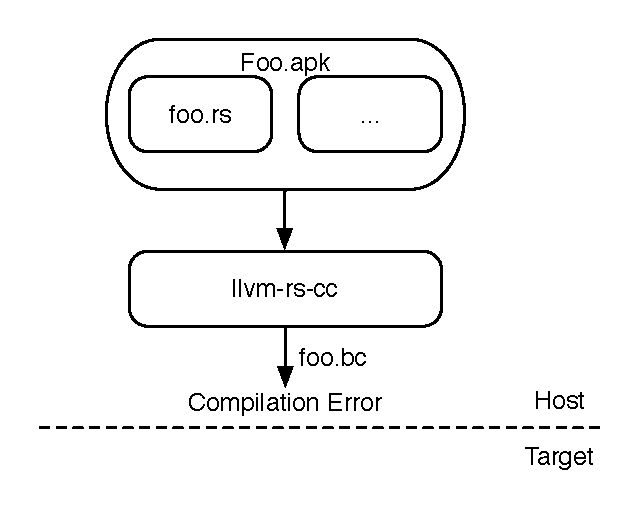
\includegraphics[scale=0.8]{fig/libbcc_workflow.eps}
	\caption{workflow of libbcc}
	\label{fig:workflow_libbcc}
\end{center-figure}

\section{Core Design Choices}
\label{s:DesignChoices}
Those three goals lead to several design trade-offs. It's these trade-offs that separate \RS{} from the existing approaches on the device, such as Dalvik or the NDK. They should be thought of as different tools intended to solve different problems.

\paragraph{Performance} runtime thread-launch management
\paragraph{Portability} NEON, fragmentation. To achieve this, the Android build tools compile your \RS{} .rs file to intermediate bitcode and package it inside your application's .apk file. On the device, the bitcode is compiled (just-in-time) to machine code that is further optimized for the device that it is running on. This eliminates the need to target a specific architecture during the development process. The compiled code on the device is cached, so subsequent uses of the \RS{} enabled application do not recompile the intermediate code.

\RS{} code is compiled and executed in a compact and well defined runtime, which has access to a limited amount of functions. \RS{} cannot use the NDK or standard C functions, because these functions are assumed to be running on a standard CPU. The \RS{} runtime chooses the best processor to execute the code, which may not be the CPU, so it cannot guarantee support for standard C libraries. What \RS{} does offer is an API that supports intensive computation with an extensive collection of math APIs. 

\paragraph{Usability} workflow, C99
 comfortable with developing in C (C99 standard) 

Usability was a major driver in \RS{} design. Most existing compute and graphics platforms require elaborate glue logic to tie the high performance code back to the core application code. This code is very bug prone and usually painful to write. The static analysis we do in \textit{llvm-rs-cc} is helpful in solving this issue. Each user script generates a Dalvik "glue" class. Names for the glue class and its accessors are derived from the contents of the script. This greatly simplifies the use of the scripts from Dalvik.



\section{RS Objects}
\label{s:RSObject}
The usage of RS objects is for graphics operation of the pipeline in figure \ref{fig:GraphicsPipeline}. We only introduces ten essential objects in this section. For full description, please refer to \cite{package-summary}.

\begin{center-figure}
    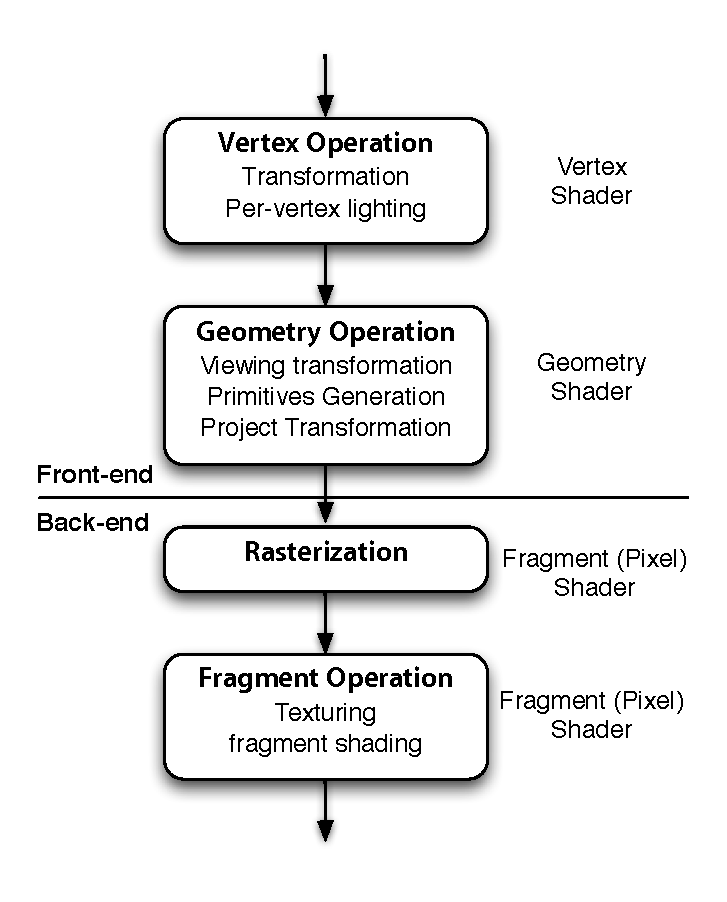
\includegraphics[scale=0.8]{fig/Graphics_Pipeline.eps}
    \caption{The typical graphic pipeline}
    \label{fig:GraphicsPipeline}
\end{center-figure}

\paragraph{Element}
An Element is the most basic element of a memory type. An element represents one cell of a memory allocation. An element can have two forms: Basic or Complex. They are typically created from C structures in your \RS{} code during the reflection process. Elements cannot contain pointers or nested arrays. The other common source of elements is bitmap formats.
A basic element contains a single component of data of any valid \RS{} data type. Examples of basic element data types include a single float value, a float4 vector, or a single RGB-565 color.

Complex elements contain a list of sub-elements and names that is basically a reflection of a C struct. You access the sub-elements by name from a script or vertex program. The most basic primitive type determines the data alignment of the structure. For example, a float4 vector is alligned to sizeof(float) and not sizeof(float4). The ordering of the elements in memory are the order in which they were added, with each component aligned as necessary.

In short, Element contains basic types and other Elements. Each entry is a type/Element and name pair. Element is very similar to C structure typedef, except no array support.

\paragraph{Type}
A collection of elements assigned a dimensional structure. For example,  R8G8B8 with height = 512, width = 256.

A Type is an allocation template that consists of an element and one or more dimensions. It describes the layout of the memory but does not allocate storage for the data that it describes. 
A Type consists of five dimensions: X, Y, Z, LOD (level of detail), and Faces (of a cube map). You can assign the X,Y,Z dimensions to any positive integer value within the constraints of available memory. A single dimension allocation has an X dimension of greater than zero while the Y and Z dimensions are zero to indicate not present. For example, an allocation of x=10, y=1 is considered two dimensional and x=10, y=0 is considered one dimensional. The LOD and Faces dimensions are booleans to indicate present or not present.

\paragraph{Allocation}
An Allocation provides the memory for applications, simply a Type with storage allocated to hold its contents. An Allocation allocates memory based on a description of the memory that is represented by a Type. The type describes an array of elements that represent the memory to be allocated. Allocations are the primary way data moves into and out of scripts.

Memory is user-synchronized and it's possible for allocations to exist in multiple memory spaces concurrently. For example, if you make a call to the graphics card to load a bitmap, you give it the bitmap to load from in the system memory. After that call returns, the graphics memory contains its own copy of the bitmap so you can choose whether or not to maintain the bitmap in the system memory. If the \RS{} system modifies an allocation that is used by other targets, it must call syncAll() to push the updates to the memory. Otherwise, the results are undefined.

Allocation data is uploaded in one of two primary ways: type checked and type unchecked. For simple arrays there are copyFrom() functions that take an array from the Android system and copy it to the native layer memory store. Both type checked and unchecked copies are provided. The unchecked variants allow the Android system to copy over arrays of structures because it does not support structures. For example, if there is an allocation that is an array n floats, you can copy the data contained in a float[n] array or a byte[n*4] array.
Script	

\paragraph{Vertex, Fragment}
The \RS{} vertex program, also known as a vertex shader, describes the stage in the graphics pipeline responsible for manipulating geometric data in a user-defined way. The object is constructed by providing \RS{} with the following data:
\begin{itemize}
    \item An Element describing its varying inputs or attributes
    \item GLSL shader string that defines the body of the program
    \item a Type that describes the layout of an Allocation containing constant or uniform inputs
\end{itemize}

The \RS{} fragment program, also known as the fragment shader, is responsible for manipulating pixel data in a user-defined way. It's constructed from a GLSL shader string containing the program body, textures inputs, and a Type object describing the constants used by the program. Like the vertex programs, when an allocation with constant input values is bound to the shader, its values are sent to the graphics program automatically. Note that the values inside the allocation are not explicitly tracked. If they change between two draw calls using the same program object, notify the runtime of that change by calling rsgAllocationSyncAll so it could send the new values to hardware. Communication between the vertex and fragment programs is handled internally in the GLSL code. For example, if the fragment program is expecting a varying input called varTex0, the GLSL code inside the program vertex must provide it.

\paragraph{Raster}
Contains the state used to rasterize primitives from Vertex programs and feed the Fragment program engine. Simply point, lines, triangles for now.
Program raster is primarily used to specify whether point sprites are enabled and to control the culling mode. By default back faces are culled.

\paragraph{Store}
Program which encapsulates the state (and possibly later programmable operations) that occur when a fragment is written to a buffer. It contains DepthTest, StencilTest, Blend, Masks, etc.

The \RS{} ProgramStore contains a set of parameters that control how the graphics hardware writes to the framebuffer. It could be used to enable and disable depth writes and testing, setup various blending modes for effects like transparency and define write masks for color components.

\paragraph{Script}
Scripts are small self-contained chunks of code that performans tasks on the programs behalf. They are compiled from C99 to llvm bitcode on the host during the build process.Several extensions to the C99 language are supported. For example, Vector types (float4, uchar4, float2, ...) and function overloading.
\begin{itemize}
\item Scripts run in a well defined environment.
\item They can only access a short list of functions.
\item They have a small fixed size stack.
\item They cannot directly share data.
\item They cannot allocate data.
\item They may call other scripts.
\item They may change the state of the rendering context.
\item They may be run concurrently with other scripts.
\item They may be run concurrently with themselves.
\end{itemize}

\RS{} scripts do much of the work in the native layer. Scripts are processed at build time. From this processing two types of Java files are generated.
\textbf{A ScriptC\_FILENAME.java} is generated for each script.  This contains code for:
\begin{itemize}
\item Initializing the script
\item Get and Set of basic global variables
\item Binding of allocation
\item Invocation of functions
\end{itemize}

\textbf{0 or more ScriptField\_typename.java} files.  These are generated for any user structures exported at pointers.
Provides an RS Element matching the structure type in the file.
\begin{itemize}
\item Error if an element cannot be created.
\item Provides packing and unpacking support to transport data from java to the RS environment.
\item Script data is broken into two categories.
\item Basic globals not declared as static
\item non pointer
\item basic types
\item generate get methods in the java class.  Initialized to same values as script.
\item If not const, generates a set method in the java class.
\item Java class caches the value from set. Sets are propagated from java to RS, however, RS updates are not propagated back to java.
\item Data updates always occur while the script is otherwise idle. 
\item Writing to globals will restrict the script to single threaded execution.
\item Pointer globals, non static.
\item Can be basic or user type.
\item User types limited to the supported set of possible elements, mostly means no arrays.
\item generate get methods in the java class initialized to null.
\item generates a bind method.  Bind point takes either an allocation for basic types or matching ScriptField\_typename object for user defined types.
\item Data updates always occur while the script is otherwise idle. 
\item Only method for writing data visible beyond the script.
\end{itemize}

\paragraph{Mesh}
A collection of allocations that represent vertex data (positions, normals, texture coordinates) and index data such as triangles and lines. Vertex data can be interleaved within one allocation, provided separately as multiple allocation objects, or done as a combination of the above. The layout of these allocations will be extracted from their Elements. When a vertex channel name matches an input in the vertex program, \RS{} automatically connects the two. Moreover, even allocations that cannot be directly mapped to graphics hardware can be stored as part of the mesh. Such allocations can be used as a working area for vertex-related computation and will be ignored by the hardware. Parts of the mesh could be rendered with either explicit index sets or primitive types.

\paragraph{Font}
This class gives you a way to draw hardware accelerated text. Internally, the glyphs are rendered using the Freetype library, and an internal cache of rendered glyph bitmaps is maintained. Each font object represents a combination of a typeface and point sizes. Multiple font objects can be created to represent faces such as bold and italic and to create different font sizes. During creation, the framework determines the device screen's DPI to ensure proper sizing across multiple configurations.

Font rendering can impact performance. Even though though the state changes are transparent to the user, they are happening internally. It is more efficient to render large batches of text in sequence, and it is also more efficient to render multiple characters at once instead of one by one.

Font color and transparency are not part of the font object and can be freely modified in the script to suit the your needs. Font colors work as a state machine, and every new call to draw text will use the last color set in the script.


\section{Memory Allocation for RenderScript}
\label{MemoryAllocation}
\begin{enumerate}
	\item Allocation = Blocks of memory for a Type 
	\item Type = Element + ArrayDims 
	\item Element = struct + name
\end{enumerate}
%Render.rs \\
%transform.rs \\
%rendernode.rs

Element, Type, Allocation, and Script. These classes are mainly used by the reflected classes that are generated from your native \RS{} code. They allocate and manage memory for your \RS{} on the Android system side. You normally do not need to call these classes directly.

\subsection{Reference Counting}
\label{refcounting}
Because of the constraints of \Core{}, you cannot do any dynamic memory allocation in your \RS{} .rs file. \Core{} can request memory from \Client{}, which allocates memory for you and does reference counting to figure out when to free the memory. A memory allocation is taken care of by the Allocation class and memory is \textbf{requested in your \RS{} code} with the the rs\_allocation type. 
All references to \RS{} objects are counted, so when your \RS{} native code or system code no longer references a particular Allocation, it destroys itself. Alternatively, you can call destroy() from \Client{}, which decreases the reference to the Allocation. If no references exist after the decrease, the Allocation destroys itself. The Android system object, which at this point is just an empty shell, is eventually garbage collected.

For example, you could manage your objects by rsSetObject() and rsClearObject()\cite{native-rs-api}.

\section{Bridge}
\label{s:Bridge}
The "physical" bridge between client side and core side is a FIFO. JNI receives the client's requests and calls the corresponded RS command to manipulate the object such as Context and Allocation at the Core side.\\
Key diagram: 
\begin{itemize}
	\item \textit{rsgAPI.cpp}: Push commands into the FIFO
	\item \textit{rsgApiReplay.cpp}: Pop commands out of FIFO
\end{itemize}
Details: Each files below contains a number that instructs rsg\_generator about the type of output (and the output will save to the filename with .rsg removed):
\\
\verb|frameworks/base/libs/rs/rsgApi.cpp.rsg|\\ 
\verb|frameworks/base/libs/rs/rsgApiFuncDecl.h.rsg|\\
\verb|frameworks/base/libs/rs/rsgApiReplay.cpp.rsg|\\ 
\verb|frameworks/base/libs/rs/rsgApiStructs.h.rsg|

\subsection{Command Queue}
\label{ss:CommandQueue}
In \RS{}, there are two kind of command queue.
\begin{itemize}
	\item \textit{mToClient}: Commands for passing message to \Client{}
	\item \textit{mToCore}: Commands to be executed in \Core{}
\end{itemize}
Note that both of them are lockless, which means atomic operation is used instead of pthread lock.

After the compilation with \slang{}, four files are generated:\\
\verb|rsgApi.cpp|\\ 
\verb|rsgApiFuncDecl.h|\\
\verb|rsgApiReplay.cpp|\\ 
\verb|rsgApiStructs.h|

\RS{} runtime commits commands through \textit{rsgApi.cpp}, take \verb|rsContextSetSurface| for example:
\begin{lstlisting}
void rsContextSetSurface (RsContext rsc, uint32_t width, uint32_t height, ANativeWindow * sur)
{
    ThreadIO *io = &((Context *)rsc)->mIO;
    RS_CMD_ContextSetSurface *cmd = static_cast<RS_CMD_ContextSetSurface *>(io->mToCore.reserve(sizeof(RS_CMD_ContextSetSurface)));
    uint32_t size = sizeof(RS_CMD_ContextSetSurface);
    cmd->width = width;
    cmd->height = height;
    cmd->sur = sur;
    // commit to the LocklessFIFO command queue
    io->mToCore.commitSync(RS_CMD_ID_ContextSetSurface, size);
};
\end{lstlisting}

The command queue keeps polling and pull the command to execute once there is any command in queue:
\begin{lstlisting}
bool ThreadIO::playCoreCommands(Context *con, bool waitForCommand) {
    bool ret = false;
    while (!mToCore.isEmpty() || waitForCommand) {
        uint32_t cmdID = 0;
        uint32_t cmdSize = 0;
        ret = true;
        if (con->props.mLogTimes) {
            con->timerSet(Context::RS_TIMER_IDLE);
        }   
        const void * data = mToCore.get(&cmdID, &cmdSize);
        if (!cmdSize) {
            // exception occured, probably shutdown.
            return false;
        }   
        if (con->props.mLogTimes) {
            con->timerSet(Context::RS_TIMER_INTERNAL);
        }   
        waitForCommand = false;
        con->timerPrint();
        if (cmdID >= (sizeof(gPlaybackFuncs) / sizeof(void *))) {
            rsAssert(cmdID < (sizeof(gPlaybackFuncs) / sizeof(void *)));
            LOGE("playCoreCommands error con %p, cmd %i", con, cmdID);
            mToCore.printDebugData();
        }   
        // execute the command 
        gPlaybackFuncs[cmdID](con, data);
        mToCore.next();
    }   

    return ret;
}
\end{lstlisting}

Then it calls the function in graphics playback function array, which is rsp prefixed:
\begin{lstlisting}
void rsp_ContextSetSurface(Context *con, const void *vp)
{
    const RS_CMD_ContextSetSurface *cmd = static_cast<const RS_CMD_ContextSetSurface *>(vp);
    rsi_ContextSetSurface(con,
           cmd->width,
           cmd->height,
           cmd->sur);
};
\end{lstlisting}

Finally, it calls the real implementation, which is rsi prefixed:
\begin{lstlisting}
void rsi_ContextSetSurface(Context *rsc, uint32_t w, uint32_t h, ANativeWindow *sur) {
    rsc->setSurface(w, h, sur);
}

\end{lstlisting}

\section{Run-time Thread-launchment in RS}
\label{s:ThreadLaunch}
Three major threads are in \RS{}.
\begin{enumerate}
\item\textbf{Context Thread} is the main thread in \Core{}
\item\textbf{Helper Thread}s are created when \textit{rsForEach()} is invoked  and the number of CPU is in direct proportion to the helper thread. 
\item\textbf{Message Thread} is used for \Core{} to deal with \Client{}.
\end{enumerate}

\subsection{Three Condition to Execute}
\label{ss:ThreeCondition}
\begin{enumerate}
	\item A surface is prepared to be drawn on.
	\item The root script\footnote{A RS script with a root function.} is compiled and binded.
	\item The RS script is for graphics rendering.
\end{enumerate}


%\subsection{Context Thread}
%\label{ss:ContextThread}
%The main thread in \Core{}
%\subsection{Helper Thread}
%\label{ss:HelperThread}
%Helper threads are created when \textit{rsForEach()} is invoked  and the number of CPU is in direct proportion to the helper thread. 
%\subsection{Message Thread}
%\label{ss:MessageThread}
%Message Thread is used for \Core{} to deal with \Client{}.
%\section{RenderScript Driver}
%\label{s:rsDriver}

%\section{Slang - LLVM RS C Compiler}
%\label{s:Slang}
%\section{Bcc - BitCode Compiler}
%\label{s:Bcc}
%\subsection{Metadata}
%\label{ss:Metadata}


